\documentclass[10pt,twocolumn]{article}

\usepackage[margin=0.75in]{geometry}
\usepackage{newtxtext,newtxmath}
\usepackage{graphicx}
\usepackage{booktabs}
\usepackage{amsmath}
\usepackage{url}
\usepackage{xurl}   % break long URLs anywhere rather than overflowing
\usepackage[hidelinks]{hyperref}
\usepackage{caption}
\usepackage{multirow}
\usepackage{listings}
\usepackage{xcolor}

% Run-in headings, defined directly: \titleformat did not take with this class
% and the headings rendered at body weight.
\newcommand{\phead}[1]{\smallskip\noindent\textbf{#1.}\hspace{0.6em}\ignorespaces}

\captionsetup{font=small,labelfont=bf,skip=4pt}
\setlength{\columnsep}{0.28in}
\setlength{\parskip}{0pt}
\setlength{\abovecaptionskip}{4pt}

\lstset{
  basicstyle=\ttfamily\scriptsize,
  breaklines=true,
  frame=single,
  rulecolor=\color{gray!50},
  backgroundcolor=\color{gray!5},
  columns=fullflexible,
  keepspaces=true,
  showstringspaces=false,
  xleftmargin=2pt,
  framexleftmargin=2pt,
}

\title{\vspace{-6mm}\textbf{Ledger: Making False Discovery Structurally Difficult\\ in Autonomous Data Analysis}\vspace{-2mm}}

\author{
Garv Bahl \quad Dhruv Kumar \quad Rahul\\
\small Department of Computer Science and Engineering\\
\small Netaji Subhas University of Technology, New Delhi, India\\
\small \texttt{\{garvbahl37\}@gmail.com}
\vspace{-4mm}
}
\date{}

\begin{document}
\maketitle

\begin{abstract}
\noindent
Language-model agents that analyse tabular data inherit a defect that predates
them: they search a large space of relationships and report the ones that look
interesting, without accounting for the size of the search. Given a table of
pure noise, where the correct number of findings is exactly zero, such a system
will confidently report several.

We present \emph{Ledger}, a multi-agent analyst built around one architectural
commitment: the language model proposes, and deterministic statistics decides.
Candidate hypotheses are registered and hashed \emph{before} any test executes,
so the family over which error is controlled is fixed before any result is seen;
test selection follows from checked assumptions rather than from model
discretion; Benjamini--Hochberg correction is applied once across the entire
registered family; and the natural-language report can only emit sentences the
statistical layer has licensed.

We evaluate on 510 synthetic tables with ground truth known by construction.
One result confirms the design and one undermines it.

First, session-level correction works. On 200 null tables an exhaustive
uncorrected analyst, which is how current agent pipelines behave, claims a false
finding on \textbf{81.0\%} of tables. The same test machinery under one
session-level correction claims one on \textbf{2.5\%}. That costs six points of
power, and the cost falls almost entirely on small effects: above $d = 0.5$ it
is under one percentage point.

Second, and less comfortably, pre-registration by a language model carries a
severe hidden cost. When the registry is supplied by the proposer rather than by
exhaustive enumeration, false discovery control becomes near-perfect (zero false
findings across 25 null tables) but power collapses to \textbf{0.13}. We localise
the failure precisely: power \emph{conditional} on a relationship having been
registered is \textbf{0.92}, while the proposer registers only \textbf{14\%} of
the relationships that exist. The statistics are working; the coverage is not.
The proposer is restricted to marginal summaries so that it cannot peek at the
data, and that same restriction leaves it with no way to tell which pairs are
worth registering. We quantify this tension and release the generators, the
harness and the system.
\end{abstract}

\section{Introduction}

Exploratory data analysis is repetitive, skilled and slow, which makes it an
obvious target for automation. Language models that write and execute code
appear to make that automation trivial: point the system at a spreadsheet and
let it report what it finds.

The appearance is misleading, for a reason older than language models. If a
relationship is declared significant at $p < 0.05$, then by construction one in
twenty tests on structureless data will pass. A table with 30 columns admits
435 pairwise relationships; roughly 22 of them will clear that threshold on pure
noise. An agent that reports what it finds will therefore always find something,
and will describe it fluently.

Human analysts are taught to guard against this with correction procedures,
pre-registration and effect-size reporting. Automated systems have inherited the
search behaviour without the discipline, and they operate at a scale that makes
the problem worse: a tireless agent can test thousands of hypotheses in the time
a human tests ten. Recent work confirms the concern is not hypothetical.
Bertran et al.~\cite{bertran2026many} show that autonomous LLM analysts
reproduce the dispersion in effect sizes and conclusions observed in human
many-analyst studies, and that the dispersion is steerable by changing the
model or the assigned persona.

\phead{The premise of this work} Statistical discipline is not a feature to
be added to an automated analyst afterwards. It has to be the thing that decides
what the analyst is allowed to say. A system that can be talked out of its
conclusions by a fluent narrative is not an analyst.

\phead{Contributions}
\begin{enumerate}\itemsep1pt
\item \textbf{An architecture in which post-hoc selection is a runtime error,
not a discouraged practice.} Hypotheses are registered and hashed before any
test executes; the registry is immutable thereafter. The family over which
error is controlled is therefore fixed before any result is visible
(\S\ref{sec:arch}).

\item \textbf{Session-level false discovery control inside the agent.}
Benjamini--Hochberg is applied once across every hypothesis registered in the
session, not per test and not per insight type.

\item \textbf{An evaluation protocol that measures whether an automated analyst
correctly reports nothing.} NULLSET and PLANTED are generated suites with
ground truth known by construction rather than by adjudication
(\S\ref{sec:protocol}).

\item \textbf{A measured decomposition of where the control comes from}, a power
curve stating what correction costs in sensitivity, and a quantification of the
coverage--validity tension that makes LLM pre-registration far more expensive
than correction alone. We did not expect the third result (\S\ref{sec:results}).
\end{enumerate}

We are explicit about what is \emph{not} new here. Benjamini--Hochberg is from
1995~\cite{benjamini1995}; pre-registration as a methodological norm is older
still. The contribution is the systems engineering that makes those ideas
binding on an autonomous agent, together with the evaluation regime that shows
it works.

\section{Related Work}

\phead{Automated analysis and insight discovery}
AutoML systems such as Auto-sklearn~\cite{feurer2015} automate model selection
but address prediction rather than explanation. Profiling tools of the
ydata-profiling lineage generate exhaustive descriptive statistics with no
notion of which findings matter; because they make no significance claims, they
have no false-discovery exposure and no way to direct attention.
QuickInsights~\cite{ding2019} introduced automatic discovery of salient patterns
and explicitly acknowledged the significance-testing problem, applying
corrections within insight types. It is the closest pre-LLM work to our concern,
though it cannot generate or execute novel analysis code.

\phead{Language-model data agents}
InsightPilot~\cite{ma2023} couples a model to an insight engine to steer
exploration; Data Interpreter~\cite{hong2024} demonstrates end-to-end agentic
data-science pipelines with code execution. Both substantially advance what such
systems can attempt. Neither controls false discovery across the exploration
session, and neither prevents post-hoc selection of hypotheses.
BLADE~\cite{gu2024blade} benchmarks agents against expert-validated analytic
decisions and documents that multiple justifiable approaches typically exist for
a single question. We return to that in \S\ref{sec:threats}, because it bounds
what any deterministic adjudicator can claim.

\phead{Per-test rigour versus session-level validity}
The closest contemporary work is Fisher-R1~\cite{miao2026fisher}, which trains
an agent by reinforcement learning for reliable hypothesis testing and
introduces P-Bench, 425 tasks in which an agent must select a method, compute a
$p$-value and draw a conclusion. Fisher-R1 targets a failure mode adjacent to
ours, namely inferential errors despite correctly executed analyses, and
improves substantially on strong baselines. It is, however, scoped to a single
hypothesis test per task, and neither its method nor its benchmark addresses
multiple comparisons across a session. The distinction matters: per-test rigour
is necessary but not sufficient. An agent that is individually correct on each
of forty tests, with no accounting for the fact that it ran forty, still
accumulates false discoveries at the rate our null experiments measure.

\phead{Detecting noise-fitting by other means}
Rewolinski et al.~\cite{rewolinski2026sanity} propose perturbation-based sanity
checks grounded in the Predictability--Computability--Stability framework, which
screen whether an agent can distinguish signal from noise and can expose
affirmative conclusions as unsupported. This is a complementary axis: theirs is
a stability argument applied after an analysis is produced, ours is a
multiplicity argument enforced before any test runs. The two compose, and we
regard combining them as the natural next step.

\phead{Statistical discipline and adaptivity}
Benjamini--Hochberg~\cite{benjamini1995} supplies the correction we apply.
False-Positive Psychology~\cite{simmons2011} demonstrated how ordinary analytic
flexibility produces significant results from nothing; the garden-of-forking-paths
argument~\cite{gelman2014} showed this occurs even absent intent to game the
analysis, which is precisely the situation of an autonomous agent. Work on
adaptive data analysis~\cite{dwork2015} bounds generalisation error under
adaptively chosen queries using differential privacy and holdout reuse. Our
approach differs in kind: rather than tolerating adaptivity and paying for it
with noise, we eliminate adaptivity by construction over the registered family.
The resulting guarantee is narrower but legible and cheap to enforce.

\phead{Execution-grounded generation}
Self-Debug~\cite{chen2024selfdebug} established that feeding execution results
back to a model improves generated-code correctness. Ledger extends the
principle from code correctness to claim correctness: execution decides not
merely whether the code ran, but whether the sentence may be written.

\section{The Ledger Architecture}
\label{sec:arch}

Ledger is a fixed, hand-written state machine over eight agents. The
orchestration is deliberately not a general-purpose agent framework: the
ordering constraint between registration and testing is a correctness property,
not a convenience, and must be inspectable. Table~\ref{tab:agents} lists the
stages and, critically, which of them involve a language model at all.

\begin{table}[t]
\centering\small
\begin{tabular}{@{}llp{3.1cm}@{}}
\toprule
\textbf{Stage} & \textbf{Model?} & \textbf{Role} \\
\midrule
A0 Janitor      & no  & Type coercion, deduplication \\
A1 Profiler     & no  & Marginal summaries only \\
A2 Proposer     & yes & Proposes testable hypotheses \\
\textbf{A3 Registrar} & \textbf{no} & \textbf{Freezes and hashes the registry} \\
A4 Executor     & yes & Writes and repairs pandas code \\
A5 Statistician & no  & Assumptions, test choice, FDR \\
A6 Reporter     & yes & Writes prose from licensed text \\
A7 Adversary    & yes & Red-teams the draft report \\
\bottomrule
\end{tabular}
\caption{The stages that decide what is true contain no language model. The
model proposes and phrases; it never adjudicates.}
\label{tab:agents}
\vspace{-4mm}
\end{table}

\subsection{The ordering constraint}

A3 runs to completion before A4 starts. Once the registry is frozen no
hypothesis may be added, and every registered hypothesis must be tested and
reported on, including those that fail. This is what makes selective reporting
impossible: the denominator of the correction is fixed before any result is
seen. An agent that could append hypotheses mid-session, or quietly drop the
disappointing ones, would invalidate the correction entirely.

The constraint is enforced at the data-model level rather than by prompt. The
registry is a field on an immutable-after-freeze object, and insertion after
freeze raises:

\begin{lstlisting}[language=Python]
def add_hypothesis(self, entry):
    if self.is_frozen:
        raise ValueError(
            "Ledger is frozen. No hypotheses can be "
            "added after A3 completes.")
    self.hypotheses.append(entry)
\end{lstlisting}

\noindent
A SHA-256 hash over the registered statements is computed at the freeze and
reported with the analysis, so a reader can verify that the family which was
corrected is the family that was registered.

\subsection{Deterministic adjudication}

A5 contains no language model. Given a hypothesis and a data slice it selects
the test from checked properties rather than from a model's suggestion:
Shapiro--Wilk and Levene decide between Welch's $t$ and Mann--Whitney $U$;
expected cell counts decide between $\chi^2$ and Fisher's exact test; for $k>2$
groups, normality and homogeneity decide between one-way ANOVA and
Kruskal--Wallis. Every result carries an effect size (Cohen's $d$, Cram\'er's
$V$, or $\eta^2$), because significance without magnitude says nothing about
whether a difference matters.

After all registered tests complete, Benjamini--Hochberg is applied once across
the entire family at $q = 0.05$. Survivors become claims; everything else is
recorded as tested-and-not-supported and appears in an appendix rather than
vanishing.

\subsection{Claim-level provenance}

Each adjudicated hypothesis yields a \texttt{licensed\_text} field, the only
text A6 may use for that hypothesis. It cannot strengthen the wording, add a
causal reading, or mention a hypothesis with no entry. In the interface, every
sentence of the report links back to the ledger entry that licensed it, so a
reader can move from any claim to the code that produced it, the assumptions
that were checked, and the test those assumptions selected.

\section{Evaluation Protocol}
\label{sec:protocol}

The clearest way to evaluate an automated analyst is to give it a dataset with
nothing in it and count what it claims to find. The correct number is zero, and
it is zero by construction rather than by judgement.

\phead{NULLSET} 200 tables, 300--2500 rows and 6--14 columns, drawn
independently. Columns carry plausible names, mixed dtypes, skewed and
heavy-tailed numerics (log-normal, gamma, bimodal, count), unbalanced
categoricals and missingness up to 12\%, so that the tables are not
distinguishable from real ones by inspection. A separate 40-table variant adds
one deterministic nuisance coupling in the form of a derived column. That
relationship is genuinely real but analytically uninteresting, and it is
recorded as ground truth so a system is not penalised for finding it.

\phead{PLANTED} 240 tables containing 2--4 genuine relationships at
controlled effect sizes $d \in \{0.2, 0.35, 0.5, 0.8\}$, buried among noise
columns. Effects are planted in three forms so that test selection is exercised
rather than a single code path: a mean shift on a binary split, a linear
association between two numerics (with $r = d/\sqrt{d^2+4}$), and a spread of
group means across a $k>2$ factor.

\phead{Arms} All arms execute the \emph{same} test-selection code, A5's
own selector. This is deliberate and is what makes the comparison meaningful:
the arms differ only in which hypotheses enter the family and whether the family
is corrected, never in how a test is chosen or computed.

\begin{itemize}\itemsep1pt
\item \textbf{Exhaustive, uncorrected.} Test every column pair; claim every
$p<0.05$. This is what an agent with code execution and no discipline does.
\item \textbf{Exhaustive, BH-corrected.} Every column pair, corrected once
across all of them. Isolates the contribution of correction alone, holding the
candidate set fixed.
\item \textbf{Registry, uncorrected} and \textbf{Registry, BH-corrected.} The
candidate set is whatever the A2 proposer registered from the marginal profile,
frozen before execution. Comparing these against the exhaustive arms separates
the effect of a \emph{smaller, model-chosen} family from the effect of
correcting across it.
\end{itemize}

Failed tests remain in the family at $p = 1.0$ rather than being dropped;
removing them would shrink $m$ and make the threshold more permissive for
everything else, which is the exact accounting error the architecture exists to
prevent.

\phead{Suite accounting} The deterministic arms run on all 480 tables
(200 NULLSET, 240 PLANTED, 40 nuisance). The registry arms re-evaluate a
50-table subset of those same tables, using the same data under a different
family, so they add no new tables. The coverage diagnostic of \S\ref{sec:coverage} uses 30
further PLANTED tables drawn from a disjoint seed range. The unique total is
therefore 510 tables, not the sum of the per-experiment counts.

\phead{Measures} We report mean findings claimed per table; the fraction of
tables on which at least one false finding is claimed (the quantity a
practitioner cares about); the false discovery proportion
$\mathrm{FDP} = \mathrm{FP}/\max(\mathrm{claims},1)$, whose expectation BH
controls; and, on PLANTED, power as recall of planted effects.

\section{Results}
\label{sec:results}

Across the suites, 23{,}901 statistical tests were executed over 23{,}909
candidate hypotheses.

\begin{figure}[t]
\centering
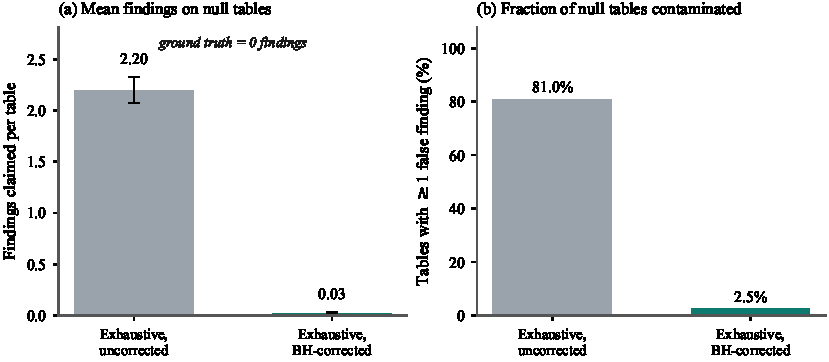
\includegraphics[width=\columnwidth]{figures/fig1_nullset.pdf}
\caption{Findings claimed on 200 tables containing no real relationships.
Ground truth is zero. Error bars are standard errors over tables.}
\label{fig:null}
\vspace{-3mm}
\end{figure}

\subsection{The null-dataset result}

Figure~\ref{fig:null} and Table~\ref{tab:main} give the headline. On tables
where the correct number of findings is zero, the uncorrected exhaustive analyst
claims $2.20 \pm 0.25$ findings per table and contaminates \textbf{81.0\%} of
tables with at least one false discovery. Applying Benjamini--Hochberg once
across the same candidate set, using the same tests on the same data, reduces
this to $0.025 \pm 0.022$ claims per table and \textbf{2.5\%} of tables. That is
a $32\times$ reduction in claims and a $98\%$ reduction in the fraction of
contaminated analyses.

We draw attention to the nuisance variant. When a single trivially-real
relationship is present, the corrected system recovers it on every table
(power $1.00$) while claiming $1.08$ things in total; the uncorrected system
recovers it too, but buries it among $3.03$ false findings. What correction
removes here is the false output, not the true one.

\begin{table}[t]
\centering\small
\setlength{\tabcolsep}{3.5pt}
\begin{tabular}{@{}llrrr@{}}
\toprule
\textbf{Suite} & \textbf{Arm} & \textbf{Claims} & \textbf{Any FD} & \textbf{FDP} \\
\midrule
\multirow{2}{*}{NULLSET}
  & uncorrected & 2.200 & 81.0\% & 0.810 \\
  & BH          & \textbf{0.025} & \textbf{2.5\%} & \textbf{0.025} \\
\midrule
\multirow{2}{*}{\shortstack[l]{NULLSET\\+nuisance}}
  & uncorrected & 4.025 & 95.0\% & 0.668 \\
  & BH          & \textbf{1.075} & \textbf{5.0\%} & \textbf{0.029} \\
\midrule
\multirow{2}{*}{PLANTED}
  & uncorrected & 5.287 & 85.8\% & 0.410 \\
  & BH          & \textbf{2.850} & \textbf{19.6\%} & \textbf{0.056} \\
\bottomrule
\end{tabular}
\caption{Mean claims per table, fraction of tables with at least one false
discovery, and mean false discovery proportion. $n=200/40/240$ tables.}
\label{tab:main}
\vspace{-4mm}
\end{table}

\subsection{What discipline costs}

\begin{figure}[t]
\centering
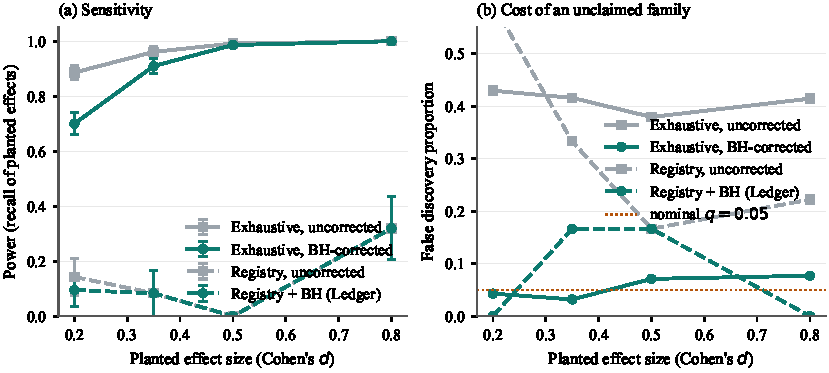
\includegraphics[width=\columnwidth]{figures/fig2_power.pdf}
\caption{Power and false discovery proportion against planted effect size on
240 PLANTED tables. The corrected arm tracks the nominal $q=0.05$ line; the
uncorrected arm sits near $0.41$ throughout.}
\label{fig:power}
\vspace{-3mm}
\end{figure}

A system that reports nothing is trivially safe and useless, so the interesting
question is what the discipline costs in sensitivity. Figure~\ref{fig:power}
answers it. Aggregated over PLANTED, correction reduces power from $0.960$ to
$0.899$, a loss of six percentage points, while reducing the false discovery
proportion from $0.410$ to $0.056$.

The aggregate understates how favourable the trade is, because the cost is
concentrated entirely at small effects:

\begin{center}\small
\begin{tabular}{@{}lrrr@{}}
\toprule
$d$ & Power (BH) & Power (unc.) & $\Delta$ \\
\midrule
0.20 & 0.700 & 0.886 & $-0.186$ \\
0.35 & 0.910 & 0.961 & $-0.051$ \\
0.50 & 0.986 & 0.992 & $-0.006$ \\
0.80 & 1.000 & 1.000 & $\phantom{-}0.000$ \\
\bottomrule
\end{tabular}
\end{center}

\noindent
At $d \geq 0.5$ correction is effectively free: it costs under one percentage
point of power and takes the false discovery proportion from $\sim$0.40 to
$\sim$0.07. The system pays for its discipline only where the signal is
genuinely faint, which is where a finding is least trustworthy anyway. We regard
this as the central practical result: the objection that statistical discipline
makes an automated analyst too conservative to be useful is, at moderate and
large effect sizes, simply not borne out.

\subsection{Empirical calibration}

The corrected arm's false discovery proportion is $0.043$, $0.032$, $0.071$ and
$0.077$ at $d = 0.2, 0.35, 0.5, 0.8$ against a nominal $q = 0.05$. That the
achieved rate sits near the nominal rate, rather than far below it, indicates
the procedure is neither broken nor gratuitously conservative on these suites.

\subsection{The cost of pre-registration}
\label{sec:coverage}

The arms above hold the candidate family fixed at every column pair. That
isolates correction, but it is not how Ledger runs: in the deployed system the
family is whatever the proposer registered. Substituting the model-chosen
registry produces the result in Table~\ref{tab:registry}, and it is not the
result we expected.

\begin{table}[t]
\centering\small
\setlength{\tabcolsep}{3.5pt}
\begin{tabular}{@{}llrrr@{}}
\toprule
\textbf{Family} & \textbf{Corr.} & \textbf{$m$} & \textbf{Any FD} & \textbf{Power} \\
\midrule
Exhaustive & no  & 51.6 & 85.8\% & 0.960 \\
Exhaustive & BH  & 51.6 & 19.6\% & 0.899 \\
Registry   & no  & \phantom{0}8.7 & 40.0\% & 0.137 \\
Registry   & BH  & \phantom{0}8.7 & \textbf{\phantom{0}8.0\%} & \textbf{0.123} \\
\bottomrule
\end{tabular}
\caption{PLANTED. A model-chosen registry drives false discovery down further
than correction alone, and takes power with it.}
\label{tab:registry}
\vspace{-4mm}
\end{table}

On null tables the registry arm is flawless: across 25 tables it claimed
\emph{zero} false findings, against 2.5\% of tables for exhaustive-plus-BH. A
smaller family is a genuinely powerful error-control mechanism, and combining it
with correction is better than either alone.

But power falls from $0.899$ to $0.123$. A system that finds one planted
relationship in eight is of little use to anyone. The natural reading is that
discipline has made the system too conservative. The instrumentation shows that
this reading is wrong. Over 30 further PLANTED tables containing 92 planted
relationships in total:

\begin{center}\small
\begin{tabular}{@{}lr@{}}
\toprule
Planted relationships & 92 \\
\dots\ the proposer \emph{registered} & 13 \ \ (14.1\%) \\
\dots\ the system then \emph{detected} & 12 \\
\midrule
Unconditional power & 0.130 \\
\textbf{Power conditional on registration} & \textbf{0.923} \\
\bottomrule
\end{tabular}
\end{center}

\noindent
Once a real relationship is in the registry, the pipeline finds it $92\%$ of the
time. Nothing is wrong with the tests, the assumption checks, or the correction.
The entire loss is upstream: the proposer registers about nine of roughly
fifty-two available pairs, and those nine are mostly not the ones that carry
signal.

\phead{Why this is not a prompt-engineering bug} It would be natural to
conclude that the proposer simply needs a better prompt. We think the problem is
structural. The proposer is shown marginal summaries \emph{only}, meaning column
types, cardinality, missingness and per-column distributions. That restriction
is what makes the correction sound. If hypothesis selection were
informed by the relationships in the data, the registry would be a
data-dependent choice and the family would no longer be fixed independently of
the results, exactly the leakage that FDR control assumes away. So the proposer
is blind by construction, and a blind proposer choosing nine pairs out of
fifty-two will cover about seventeen percent of the space regardless of how
well it is prompted.

We call this the coverage--validity tension. Withholding the relationships from
the proposer is what lets us treat the registry as fixed independently of the
results, and it is also why the proposer cannot tell a promising pair from an
unpromising one. Any system that pre-registers hypotheses through a model that
has not seen the relationships will face some version of the same problem.

\phead{What this implies} We read the tension as a budgeting problem, and
three directions follow from it. The registration budget can be raised:
registering thirty pairs instead of nine buys much better coverage at the price
of a more conservative threshold, and because BH scales gracefully in $m$ that
price is low. Domain knowledge, supplied
through the data dictionary rather than through the data, raises coverage
without creating leakage, which is an argument for the RAG path the system
already has. Sample splitting is the most promising of the three: a proposer could see
relationships in one partition and register hypotheses to be tested on another,
recovering coverage while keeping the family independent of the data it is
evaluated on. That is the adaptive data analysis setting~\cite{dwork2015}, and
connecting the two properly is the clearest next step for this work.

\section{Threats to Validity}
\label{sec:threats}

\phead{Synthetic nulls may be easier than real ones} Real data contains
genuine but uninteresting structure, such as encoding artefacts and collection
effects, that independently drawn columns lack. Our nuisance variant is a
partial mitigation and shows the corrected system handles one such coupling
correctly, but a stronger test is permuted real datasets, which preserve
marginal distributions while destroying relationships. We have not yet run that
and do not claim its result.

\phead{FDR control assumes the registry is the full family} If the
proposer's choice of hypotheses is itself informed by peeking at the data, the
correction is optimistic. The profiler's output is deliberately restricted to
marginal summaries for this reason, and the restriction is enforced in code
rather than requested in a prompt. We have not measured the residual leakage,
and we flag it as the most important open question about the guarantee.

\phead{The main experiment isolates correction, not the full architecture}
The two arms reported here share a candidate set and differ only in correction.
This cleanly establishes what correction contributes but does not, on its own,
establish what \emph{pre-registration} contributes over and above it. A
proposer-driven arm is required for that, and is discussed in
\S\ref{sec:limits}.

\phead{Deterministic does not mean uniquely correct}
BLADE~\cite{gu2024blade} documents that experts frequently disagree about the
right analysis for a given question. Our claim for A5 is therefore that test
choice is \emph{reproducible and inspectable}, not that it is the only
defensible choice. Where assumptions do not resolve cleanly, the selected test
and the checks that selected it are both recorded.

\phead{Results are implementation-dependent} All arms share one test
implementation. This is a strength for internal validity and a limit on external
validity: a different statistics stack might shift absolute numbers, though the
direction of the comparison does not depend on it.

\section{Limitations and Future Work}
\label{sec:limits}

The registry arms are run at $n=25$ null and $n=55$ planted tables against
$n=480$ for the deterministic arms, because each costs a model call. The
coverage figure of \S\ref{sec:coverage} is therefore the least precisely
estimated number in the paper, and the one most worth re-running at scale. Its
direction is not in doubt, since a proposer that registers nine of fifty-two
pairs cannot have high coverage, but the point estimate should be read with that
sample size in mind.

We evaluate one proposer model. Coverage is plausibly model-dependent in a way
that correction is not, so the $14\%$ figure should be read as a measurement of
this configuration rather than a constant of nature.

Four extensions follow directly. First, the registration-budget sweep of
\S\ref{sec:coverage}, which is cheap and would turn the tension we report into a
dose--response curve. Second, sample splitting to break the tension outright,
connecting this work to adaptive data analysis~\cite{dwork2015}. Third,
evaluation on an external benchmark: P-Bench~\cite{miao2026fisher} is the
natural target, extended so that multiple tasks are bundled into one session,
which would test session-level validity on data we did not generate. Fourth,
composing our multiplicity argument with the stability argument of Rewolinski et
al.~\cite{rewolinski2026sanity}; the two screen for different failures and
neither subsumes the other.

\section{Conclusion}

Automated analysts have inherited the search behaviour of human exploratory
analysis without its discipline. We have shown that the discipline can be made
architectural rather than advisory, and that doing so takes the fraction of null
tables yielding a false finding from 81.0\% to 2.5\% at a cost in power that is
negligible above $d = 0.5$.

The two mechanisms are not equally cheap. Correction is close to free.
Pre-registration through a blind proposer costs roughly seven-eighths of the
system's power in our configuration, and it does so because the proposer covers
$14\%$ of the search space rather than because the statistics are too strict.
That is the more useful of the two findings, since it says where the next
improvement has to come from. A version of this paper without it would have
described a system that controls false discovery well and finds almost
nothing.

The system, the generators and the harness are available at
\url{https://github.com/garvbahl37-gif/Ledger_agent}.

\begin{thebibliography}{99}\small
\setlength{\itemsep}{0pt}

\bibitem{benjamini1995}
Y.~Benjamini and Y.~Hochberg.
\newblock Controlling the false discovery rate: a practical and powerful
approach to multiple testing.
\newblock {\em J. Royal Statistical Society B}, 57(1):289--300, 1995.

\bibitem{bertran2026many}
M.~Bertran, R.~Fogliato, and Z.~S. Wu.
\newblock Many {AI} analysts, one dataset: navigating the agentic data science
multiverse.
\newblock {\em arXiv:2602.18710}, 2026.

\bibitem{chen2024selfdebug}
X.~Chen, M.~Lin, N.~Sch\"arli, and D.~Zhou.
\newblock Teaching large language models to self-debug.
\newblock In {\em ICLR}, 2024.

\bibitem{ding2019}
R.~Ding, S.~Han, Y.~Xu, H.~Zhang, and D.~Zhang.
\newblock {QuickInsights}: quick and automatic discovery of insights from
multi-dimensional data.
\newblock In {\em ACM SIGMOD}, 2019.

\bibitem{dwork2015}
C.~Dwork, V.~Feldman, M.~Hardt, T.~Pitassi, O.~Reingold, and A.~Roth.
\newblock Preserving statistical validity in adaptive data analysis.
\newblock In {\em ACM STOC}, 2015.

\bibitem{feurer2015}
M.~Feurer, A.~Klein, K.~Eggensperger, J.~Springenberg, M.~Blum, and F.~Hutter.
\newblock Efficient and robust automated machine learning.
\newblock In {\em NeurIPS}, 2015.

\bibitem{gelman2014}
A.~Gelman and E.~Loken.
\newblock The statistical crisis in science.
\newblock {\em American Scientist}, 102(6):460--465, 2014.

\bibitem{gu2024blade}
K.~Gu, R.~Shang, R.~Jiang, K.~Kuang, R.-J. Lin, D.~Lyu, Y.~Mao, Y.~Pan, T.~Wu,
J.~Yu, Y.~Zhang, T.~M. Zhang, L.~Zhu, M.~A. Merrill, J.~Heer, and T.~Althoff.
\newblock {BLADE}: benchmarking language model agents for data-driven science.
\newblock In {\em EMNLP}, 2024. arXiv:2408.09667.

\bibitem{hong2024}
S.~Hong et~al.
\newblock Data interpreter: an {LLM} agent for data science.
\newblock {\em arXiv:2402.18679}, 2024.

\bibitem{ma2023}
P.~Ma, R.~Ding, S.~Han, and D.~Zhang.
\newblock {InsightPilot}: an {LLM}-empowered automated data exploration system.
\newblock In {\em EMNLP (System Demonstrations)}, 2023.

\bibitem{miao2026fisher}
J.~Miao, J.~Mu, G.~Chen, and J.~Zou.
\newblock {Fisher-R1}: training {LLM} agents for reliable hypothesis testing.
\newblock {\em arXiv:2608.07437}, 2026.

\bibitem{rewolinski2026sanity}
Z.~T. Rewolinski, A.~V. Zane, H.~Huang, C.~Singh, C.~Wang, J.~Gao, and B.~Yu.
\newblock Sanity checks for agentic data science.
\newblock {\em arXiv:2604.11003}, 2026.

\bibitem{simmons2011}
J.~Simmons, L.~Nelson, and U.~Simonsohn.
\newblock False-positive psychology: undisclosed flexibility in data collection
and analysis allows presenting anything as significant.
\newblock {\em Psychological Science}, 22(11):1359--1366, 2011.

\end{thebibliography}

\end{document}
